\Huge\textbf{Capitolo 8: \\Traffico vescicolare}\\

\small
\section{Reticolo endoplasmatico, Golgi e Lisosoma}
    Il RE è in diretta continuità con la membrana nucleare e comunica fortemente con il Golgi. Il trasporto tra RE e Golgi è mediato da vescicole. Dal RE si spostano le proteine mature pronte ad essere modificate o esportate dal Golgi.\\
    Se la proteina non possiede sequenze particolari (viste nel capitolo precendente) vengono veicolare dal RE al Golgi.
    Per trasporto anterogrado di una proteina di intende il trasporto da RE, passando per Golgi per essere poi espulsa dalla membrana.\\
    Per trasporto retrogrado si intende il percorso contrario e avviene per una determinata classe di proteine.
    
    \subsection{Golgi}
        Il Golgi è costituito da cinque cisterne (più grande delle vescicole stesse) che prendono nomi diversi in base alla propria posizione. A partire dal quella prossima al RE sono:
        \begin{itemize}
            \item Cis Golgi Network (CGN)
            \item Cis Golgi (CG)
            \item Media Golgi (MG)
            \item Trans Golgi (TG)
            \item Trans Golgi Network (TGN)
        \end{itemize}
        Essendo prossima alla membrana plasmatica, TGN è la cisterna che funge da "smistatore" per le vescicole in uscita dalla cellula (o comunque le sostanze arrivate fino a lì) generando vescicole diverse per destinazione diverse. 
        Determina l'identità del compartimento di destinazione.\\
        Il contenuto di una vescicola da cisterna a cisterna muta gradualmente, non abbiamo la generazione di nuove vescicole mano a mano. Muta invece la composizione chimica interna.
        \begin{figure}[h]
            \centering
            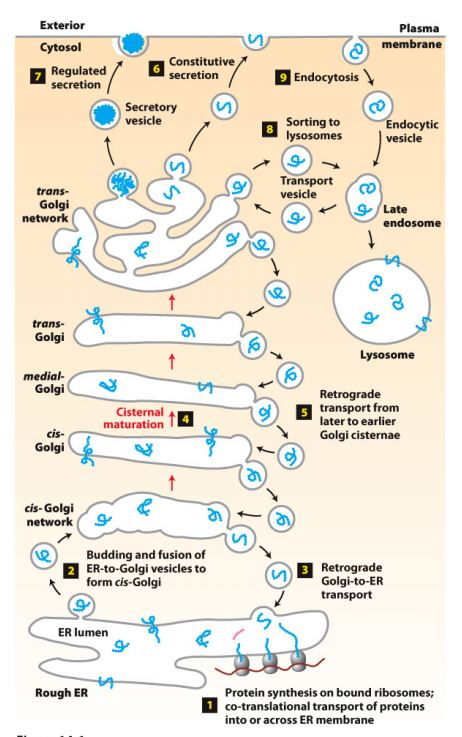
\includegraphics[width=0.5\textwidth]{images/Golgi.JPG}
            \caption{\small Schema della struttura del Golgi, si noti come TGN è deputata alla realizzazione di diverse tipologie di vescicole}
            \label{fig:mesh1}
        \end{figure}
            \subsubsection{Funzioni}
            Il Golgi è adibito alla glicosilazione delle proteine. Questo processo inizia nel CGN e la modifica prende parte in cisterne diverse con step graduali fino ad arrivare al TGN. \\
            Il Golgi contiene delle proteine residenti quali glicosidasi e glicosiltransferasi per adempiere alla propria funzione di glicosilare i peptidi.
            
    \subsection{Lisosoma}
        Il lisosoma è un componente cellulare vescicolare che si occupa della degradazione di materiali per lo più extracellulari, batteri o organelli non più in grado si svolgere il proprio compito. Ha quindi una funzione catabolica. La fusione dell'endosoma tardivo con un lisosoma determina la degradazione del suo contenuto.\\
        Il lisosoma possiede un pH acido per consentire alle idrolasi acide di svolgere il proprio compito, per questo motivo presenta delle pompe protoniche per mantenere questo livello di acidità. 
            
    \subsection{Esperimenti}
        \subsubsection{VSV-G}
            L'obiettivo è visualizzare la proteina virale VSV-G (proteina di superficie) che da neosintetizzata di trova nel RE. Dopo 40 minuti si ritrova nel Golgi mentre dopo 30 ore si trova nella membrana.\\ 
            Per fare ciò viene utilizzata una GFP, una proteina naturale che riesce a effettuare un processo di bioluminescenza.\\
            La cellula produce VSV-G in un singolo istante perchè la proteina (modificata, non wt) è sensibile alla temperatura. Quindi questa variante è più prona a non ripiegarsi correttamente a una temperatura più elevata del normale (\textit{temperatura non permissiva}). 
            Qualora la proteina non fosse ripiegata correttamente non viene trasportata.\\
            Le cellule vengono spostate alla temperatura permissiva, la proteina ri ripiega correttamente e viene rilasciata dal RE verso il Golgi e via dicendo.
            
        \subsubsection{Mutanti deficitari}
            I mutanti deficitari sono mutanti con impedimenti di specifiche funzioni coinvolte nei processi interposti tra la sintesi e l'espulsione dalla membrana. \\
            Sono stati ampiamente utilizzati tramite cellule di lievito. Queste funzioni sono essenziali per la vita, di conseguenza sono stati selezionati mutanti temperatura sensibili.\\
            La classe di mutanti A, posti alla temperatura non permissiva accumulano proteine secretorie nel citosol, quindi la funzione difettiva consisteva nell'importo nell'ER (mutanti SEC).\\
            Altre classi di mutanti accumulano proteine nel lumen dell'ER (deficit nella gemmazione), accumulano proteine nelle vescicole di connessione ER - Golgi, accumulo nel Golgi.\\
            Incrociando mutanti diversi si possono osservare fenotipi che sono stati essenziali allo studio di questi eventi.

\section{Gemmazione e fusione}
    \subsection{Coat Proteins}
        La gemmazione delle vescicole è guidata dalle Coat Proteins (CP). Sono queste proteine a dettare una curvatura della membrana associandosi ad essa.\\
        Le CP hanno interazioni specifiche con proteine trans membrana e GTPasi associate. La deformazione della membrana determina la formazione di una protrusione che alla fine si distaccherà.
        Una volta che la vescicola è stata formata si procede a un disassemblaggio delle CP prima che essa arrivi alla propria destinazione.\\
        Esistono vari tipi di CP, i quali determinano la tipologia delle vescicole:
        \begin{itemize}
            \item COP1 (con ARF): impiegata nel trasporto retrogrado. ARF è una GTP binding-protein.
            \item COP2 (con SAR1): impiegata nel trasporto anterogrado. SAR1 è una GTPasi che induce gemmazione qualora sia associata al foglietto citosolico e recluta membri di COP2 per la vescicolazione, nel momento in cui il GTP viene idrolizzato si induce il distacco dei COP1.
            \item Clatrina (con ARF)
        \end{itemize}
        SAR1 e ARF sono presenti a livello citoplasmatico associate a GDP quindi inattive.\\
        Non è nota la CP specifica per il trasporto da TGN alla membrana cellulare.\\
        Vari esperimenti hanno confermato la necessaria presenza delle CP per la formazione delle vescicole e della necessità di avere un'idrolisi di GTP per il rilascio del coat (per il secondo esperimento si utilizza GTP$\gamma$s il quale non permette idrolisi).
        
    \subsection{Gemmazione con COP2}
        A livello citoplasmatico SAR1 è libera finchè SEC12 non interagisce come GEF: SAR1 viene "caricata" con GTP facendo esporre il proprio N-terminale idrofobo. Questo fa sì che SAR1 si associ al foglietto citosolico della membrana. \\
        Questa associazione determina la recluta di altri componenti proteici di COP2 che vanno a formare la vescicola. Nel momento in cui il GTP di SAR1 viene idrolizzato (GAP), il coat si disassembla e la vescicola rimane nuda.
        
    \subsection{Clatrina}
        La clatrina è un dipeptide, tre di questi dipeptidi formano una struttura a triscele. 36 trisceli formano una struttura sferica attorno a una vescicola. 
        La clatrina non sa interagire autonomamente con la vescicola, ma ha bisogno di un'adattina, una proteina che consente l'interazione con la membrana.\\
        Il distacco della vescicola che si forma in presenza della clatrina è operata dalla dinamina. La dinamina è una proteina che opera una "strozzatura" del collo della gemma corrispondente alla nuova vescicola e ne determina il distacco effettivo. La dinamina è di per sè una GTPasi multimerica, di conseguenza questo processo energicamente sfavorito è realizzabile spendendo GTP. 
        Non si conoscono proteine analoghe per gli atri tipi di CP.
    
    \subsection{Adattina}
        Le adattine (adapter proteins) sono una classe di proteine che aiutano la clatrina a formare la struttura sferica per la vescicola (per esempio AP1, GGA e AP2).\\
        Un particolare adattina riesce anche interagire direttamente con la vescicola e formare un coat autonomo in assenza della clatrina (AP3 complex).
        
        
    \subsection{Fusione}
        La fusione della vescicola con CGN avviene grazie all'interazione di proteine specifiche chiamate\textbf{ V-SNARE}, presenti sulla vescicola, e \textbf{T-SNARE}, presenti sulla membrana target.\\
        Entrambe le SNARE sono proteine costituite da coiled coil specificamente molto affini tra loro. La loro interazione promuove la giustapposizione dei foglietti citosolici. 
        L'avvicinamento e la fusione delle membrane non è un processo energicamente favorito, tuttavia l'interazione delle proteine citate sopra, consente di superare la barriera energetica e di compiere la fusione.\\
        L'esposizione delle V-SNARE avviene dopo la perdita delle CP. Esistono circa 20 diverse tipologie di V e T-SNARE specifiche per l'interazione di determinate membrane di origine con determinate membrane target.\\
        La dissociazione dei coiled coil che si formano per la fusione richiede energia, per questono intervengono delle AAA-ATPasi.\\
        
        In particolare, le V-SNARE presenti su TGN sono chiamate VAMP mentre le T-SNARE della membrana sono sintaxina e SNAP25. La fusione alla membrana plasmatica avviene attraverso l'interazione di 4 polipeptidi (VAMP, sintaxina e due molecole di SNAP25).\\
        
        A livello vescicolare è presente anche una GTPasi della famiglia delle \textit{RAB}. Ogni RAB caratterizza una membrana di origine e determina specificità con la destinazione. 
        Le RAB hanno un ciclo specifico di associazione a GTP e GDP, qualora la vescicola sia "in cerca" della membrana target è associata al GTP. GEF e GAP si occupano del cambio dell'attività delle RAB.
        \begin{figure}[h]
            \centering
            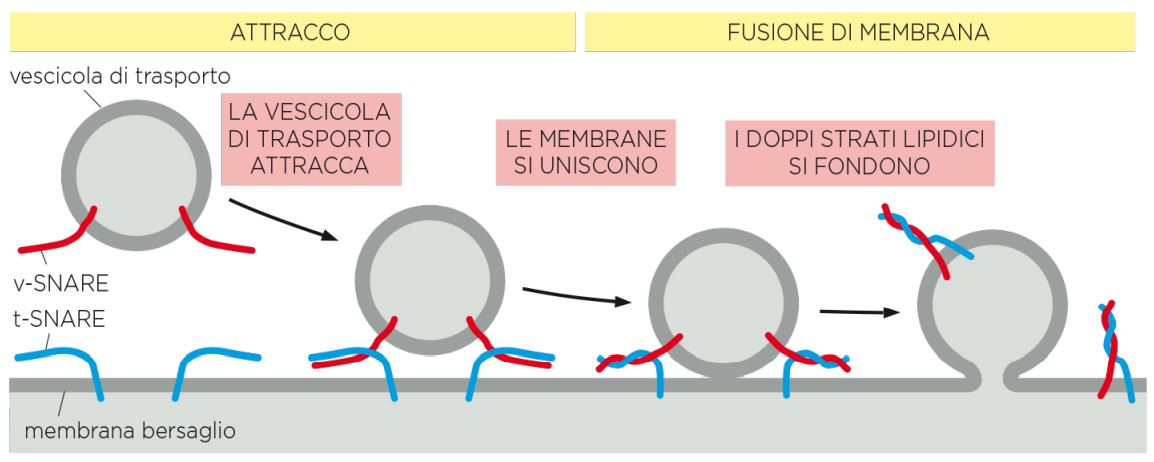
\includegraphics[width=0.8\textwidth]{images/VTSNARE.JPG}
            \caption{\small Interazione T-SNARE e V-SNARE}
            \label{fig:mesh1}
        \end{figure}
    
\section{Trasporto RE - CGN}
    Le proteine presenti sulla membrana interagiscono con componenti esterni per la formazione del coat, tuttavia esistono anche elementi proteici che si interfacciano con l'interno della vescicola con i cargo solubili. \\
    Come è facile immaginare, è proprio in dipendenza del cargo che una vescicola avrà un certo target.
    \subsection{Proteine e COP2}
        Come visto in precedenza, la formazione di del coat tramite COP2 avviene con il fine di avviare un trasporto anterogrado. \\
        La formazione del coat avviene grazie alla presenza di due SEC (23 e 24) che fungono da etichetta specifica per il target da RE a Golgi. SEC24 lega una coda proteica della proteina di membrana del RE (serve comunque l'interazione con SAR1-GTP).\\
        La coda di AA segnale esposta sul lato citoplasmatico che viene legata determina l'interazione con le proteine per il coating.\\
        Dopo questo passaggio saranno reclutati gli altri membri proteici per la formazione del coat.
        
    \subsection{Proteine e cargo solubili}
        Le proteine solubili cargo hanno sequenze AA specifiche per l'interazione con il recettore di riferimento.
        \subsubsection{Sequenza KDEL e trasporto retrogrado}
            La sequenza KDEL (lisina, asparagina, acido glutammico e leucina) è una sequenza segnale posta al C-terminale del cargo solubile tipica delle proteine luminali del RE.\\ 
            Questa sequenza codifica il fatto che la proteina deve rimanere nel lumen del RE.\\
            La sequenza KDEL possiede un recettore presente sulla membrana del Golgi: infatti nel caso in cui la proteina venga inclusa per caso in una vescicola e arrivi al Golgi, questa verrà identificata dal suo recettore che indurrà la formazione di una nuova vescicola che compierà del lavoro retrogrado per riportare la proteina con KDEL nel RE. 
            La vescicola che torna verso il RE sarà ricoperta da COP1. \\
            Una volta che la vescicola che viaggia dal Golgi verso il RE si è fusa con la membrana del RE, il recettore per KDEL si troverà associato alla membrana del RE. Tuttavia, la proteina con KDEL non interagirà con il suo recettore perchè l'associazione dipende dal gradiente protonico. Il Golgi ha una concentrazione di H$^{+}$ più elevata rispetto al RE, il quale pH induce in cambio di carica da parte della sequenza KDEL che si associa al suo recettore.
            Nel RE, il pH è più alto e questa associazione non avviene.\\
            Lo chaperon BiP è un esempio di proteina con sequenza KDEL.
            \begin{figure}[h]
                \centering
                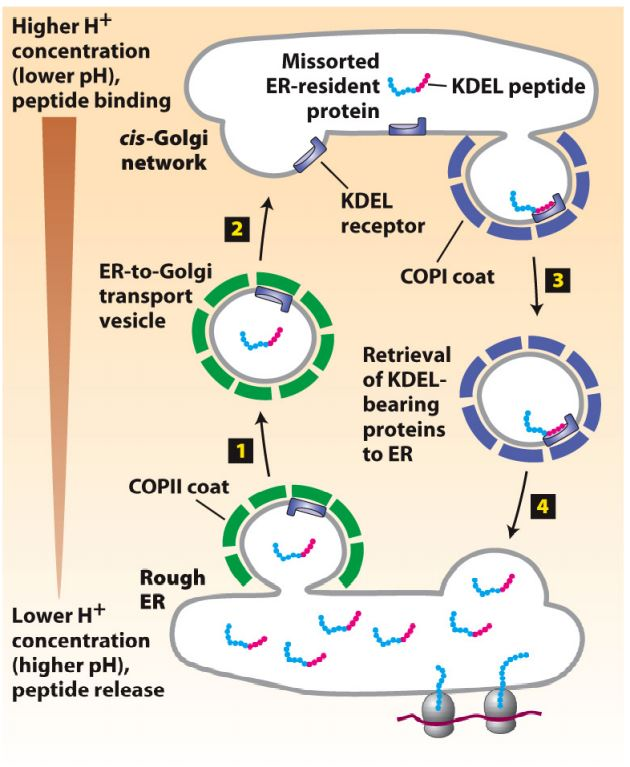
\includegraphics[width=0.5\textwidth]{images/KDEL.JPG}
                \caption{\small Trasporto erroneo anterogrado di proteina con KDEL e conseguente trasporto retrogrado}
                \label{fig:mesh1}
            \end{figure}

\section{Trasporto tra le cisterne del Golgi}
    Le cisterne del Golgi hanno contenuto e funzioni diverse in base alla loro locazione. Nel momento in cui una vescicola transita attraverso le cisterne cambia gradualmente chimicamente, seguendo un climax dettato dalle cisterne stesse.\\
    In senso anterogrado, la cisterna matura interamente senza gemmazione e fusione.\\
    In senso retrogrado c'è vescicolazione.

\section{Smistamento destinazioni del TGN}
    Il TGN, come detto in precedenza, svolge la funzione di indirizzare vescicole diverse a in direzioni specifiche. In particolare ci sono cinque path possibili che una vescicola può intraprendere:
    \begin{enumerate}
        \item esositosi costitutiva (tramite membrana)
        \item esocitosi specifica (tramite membrana)
        \item lisosoma, con APcomplex
        \item trasporto retrogrado, con COP1
        \item endosoma tardivo (ET) con Clatrina e APcomplex
    \end{enumerate}
    In alcune cellule con tipologie di membrana plasmatica ben differenziate (come le cellule epiteliali), il TGN riesce a direzionare vescicole diverse con cargo diverse per membrane diverse. 
    Lo studio di questo fenomeno è stato condotto utilizzando due virus diversi (HA dell'influenza e VSV-G) che vengono direzionate a due membrane opposte: questo suggerisce che le proteine hanno racchiuso in se stesse i segnali per essere veicolate alla membrana corretta.
    
    \subsection{Targeting del lisosoma}
        Anche le proteine solubili che devono risiedere nel lisosoma possiedono un segnale specifico: possiedono in particolare un gruppo mannosio 6-fosfato legato a una catena di glicosilazione posta in prossimità all'N-terminale (glicosilazione avviene nel CG).
        Presentano questo tipo di struttura le proteine che devono rimanere confinate nel lisosoma per garantirne la funzionalità come gli enzimi lisosomali.\\
        Di seguito il procedimento per trasportare queste proteine al lisosoma:
        \begin{enumerate}
            \item Il segnale viene letto da un recettore specifico per mannosio 6P del TGN
            \item Si forma la vescicola (clatrina)
            \item La vescicola perde le CP (clatrina)
            \item Fusione con ET
            \item ET promuove eventi di fusione per l'accesso al lisosoma
        \end{enumerate}
        Esistono delle molecole con dei marker di mannosio-6P a livello esocellulare per recuperare sostanze che sono finite erroneamente fuori dalla cellula (utilizzando lo stesso recettore), questo stesso pathway promuove la formazione di vescicole coperte da clatrina con dinamina. 

\section{Endocitosi di LDL}
    L'endocitosi è un processo che viene effettuato tramite vescicole di clatrina, AP2 e dinamina.\\
    La regolazione dell'associazione al recettore AP2 può avvenire anche in assenza del ligando nonostante l'associazione sia più stabile e duratura qualora esso sia presente. Queste vescicole possono veicolare diversi carghi, quindi sono presenti molti recettori.  \\
    Per LDL (low density lipoprotein) è destinato a essere degradato dal lisosoma per rendere disponibili i singoli componenti molecolari alla cellula. 
    LDL possiede un recettore specifico ApoB (Apolipoprpteina B) che presenta un cuore altamente idrofobico per legare le componenti lipidiche di LDL (colesterolo e trigliceridi) e un segnale per il recettore. \\
    Sarà il pH a determinare l'associazione tra ApoB e il suo recettore, in particolare:
    \begin{itemize}
        \item nel caso di pH neutro il braccio legante si associa a ApoB
        \item nel caso di pH acido (ET) il braccio si ripiega su se stesso impedendo il legame con ApoB
    \end{itemize}
    L'endocitosi di LDL è determinata da una sequenza target di AA comune per i componenti molecolari che sono destinati all'endocitosi. \\
    Persone con ipercolesterolemia (non dovute direttamente a una dieta malsana) hanno un recettore per ApoB che non riconosce la sequenza corretta, impedendo la corretta encoditosi di LDL.

\section{Degradazione lisosomiale}
    Le proteine che devono essere degradate tramite un lisosoma possono accedervi secondo due vie: la prima interessa le proteine trans-membrana che possono essere degradate o diventare componente della membrana del lisosoma, la seconda interessa componenti solubili citosolici  (ovvero il processo di autofagia).
    
    \subsection{Proteine trans-membrana}
        \subsubsection{Proteine destinate alla degradazione}
            Queste proteine sono quelle che sono state precedentemente mono-UB, processo catalizzato da complessi proteici chiamati ESCRT assieme a ATPasi e VPS4.
            Le proteine destinate alla mera degradazione interagiscono con clatrina e AP2. Nell'ET avviene la formazione di molteplici vescicole (il cui interno è porzione di citoplasma) che contengono tali proteine. 
            Nel momento in cui avviene la fusione con il lisosoma, le vescicole si ritroveranno nell'ambiente acido, la membrana verrà disciolta e con essa anche la proteina.
        \subsubsection{Proteine destinate alla membrana del lisosoma}
            Le proteine destinate alla membrana del lisosoma non vengono incluse nelle vescicole che si formano all'interno dell'ET, ma rimangono invece sulla membrana estrerna. Al momento della fusione, la membrana dell'ET si fonde con quella del lisosoma e le proteine in questione faranno ora parte della membrana del lisosoma.
        \begin{figure}[h]
            \centering
            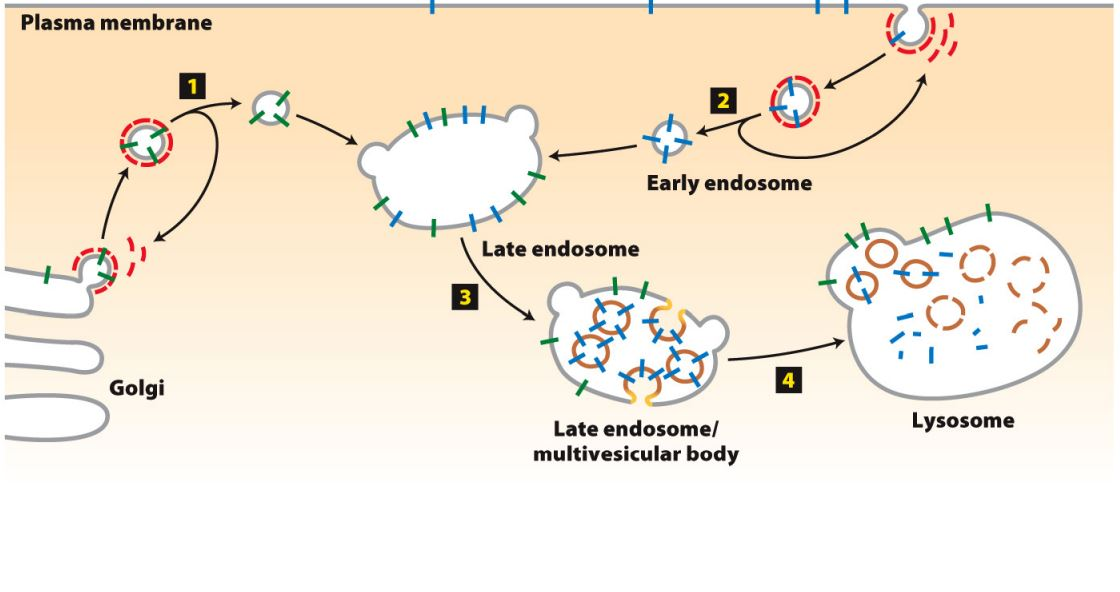
\includegraphics[width=1\textwidth]{images/degradazioneLisosoma.JPG}
            \caption{\small Proteine destinate alla degradazione in blu, proteine destinate alla membrana del lisosoma in verde}
            \label{fig:mesh1}
        \end{figure}
    \subsection{Componenti cistosolici solubili}
        Il processo di degradazione di componenti citosoloci solubili è detto anche autofagia. Questo processo è coinvolto in diverse situazioni: 
        \begin{enumerate}
            \item degradazione di componenti cellulari vecchi o non funzionanti
            \item degradazione di altri contenuti proteici presenti nel citosol
            \item degradazione di porzioni citosoliche in caso di carenze metaboliche
        \end{enumerate}
        I polipeptidi coinvolti nel processo di autofagia (1 e 3) sono i medesimi. In particolare analizzando il caso del lievito, si nota che sono presenti una famiglia di proteine chiamata ATG (autophagy) di cui in particolare fa parte ATG8. 
        ATG8 (nelle cellule umane l'analoga è chiamata LC3) è un peptide presente in due forme: solubile e associato alla membrana (quindi con componente lipidica). 
        ATG8 coopera con le membrane pre-esistenti per la formazione di una "capsula" a doppio strato fosfolipidico attorno alla porzione di citosol/organello da degradare chiamata \textit{autofagosoma}.\\
        L'autofagosoma viene quindi incluso nel lisosoma e ne viene degradato il contenuto.
        \begin{figure}[h]
            \centering
            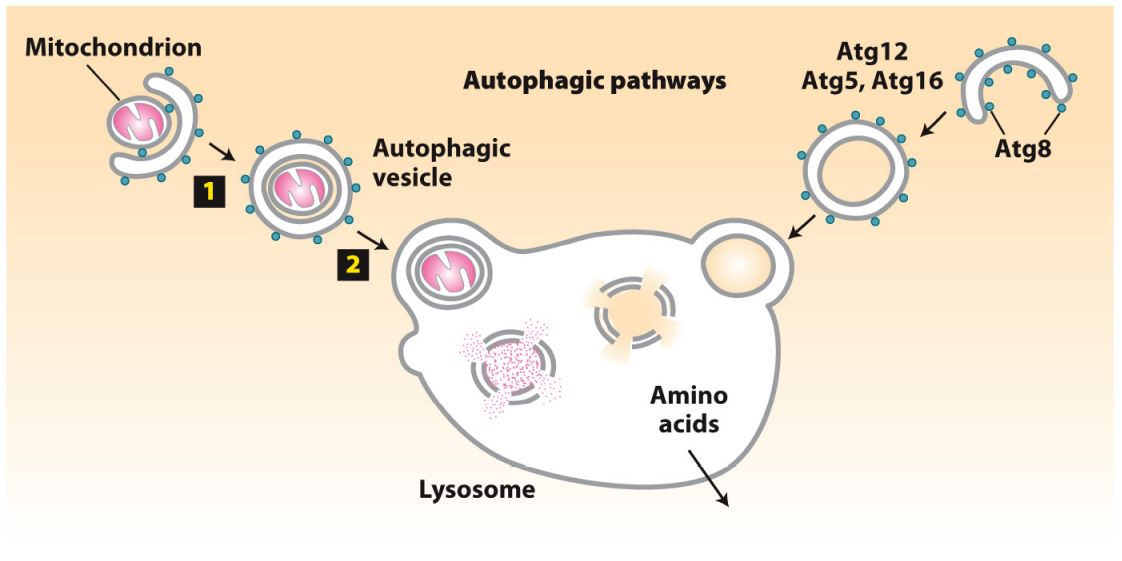
\includegraphics[width=1\textwidth]{images/Autofagia.JPG}
            \caption{\small Processo di autofagia per un organello e per porzioni di citoplasma}
            \label{fig:mesh1}
        \end{figure}
        
\pagebreak
